\documentclass[xcolor=table]{beamer}

\mode<presentation> {
\usetheme{CambridgeUS}}
\usepackage[utf8]{inputenc}
\usepackage{booktabs}
\usepackage{fixltx2e}
\usepackage{graphicx} % Allows including images
\usepackage{listings}
\usepackage{color}
\usepackage{soul}
\definecolor{important}{rgb}{0.08, 0.38, 0.74}
\definecolor{amber}{rgb}{0.94,1.0,0.94}
\definecolor{columbiablue}{rgb}{0.94,1.0,1.0}
\definecolor{carnationpink}{rgb}{0.99,0.76,0.8}
\definecolor{grannysmithapple}{rgb}{0.74,0.83,0.9}
\definecolor{britishracinggreen}{rgb}{0.0, 0.26, 0.15}
\lstdefinestyle{numbers} {captionpos=b,tabsize=2,frame=lines,keywordstyle=\color{blue},commentstyle=\color{britishracinggreen},stringstyle=\color{red},numbers=left,numberstyle=\tiny,numbersep=5pt,breaklines=true,showstringspaces=false,basicstyle=\footnotesize,emph={label}t}
\lstdefinestyle{UmpleInFrame}{backgroundcolor=\color{grannysmithapple},frame=shadowbox}
\lstdefinestyle{UmpleOutFrame}{backgroundcolor=\color{columbiablue},frame=shadowbox}
\lstdefinestyle{JavaFrame}{backgroundcolor=\color{amber},frame=shadowbox}
\lstdefinestyle{DroolsFrame}{backgroundcolor=\color{carnationpink},frame=shadowbox}

\lstdefinestyle{JavaStyle} {language=Java,style=numbers,style=JavaFrame,frame=lines}
\lstdefinestyle{UmpleInStyle} {language=Java,style=numbers,style=UmpleInFrame,frame=lines, morekeywords={isA, depend,const, after, lazy, immutable,namespace }}

\lstdefinestyle{UmpleOutStyle} {language=Java,style=numbers,style=UmpleOutFrame,frame=lines,morekeywords={isA, depend,const, after, lazy, immutable,namespace }}
\lstdefinestyle{DroolsStyle} {language=Java,style=numbers,style=DroolsFrame,frame=lines,morekeywords={when, rule, end, insert, then}}
\usepackage{tabularx}
%\usepackage{booktabs} % Allows the use of \toprule, \midrule and \bottomrule in tables

%----------------------------------------------------------------------------------------
%	TITLE PAGE
%----------------------------------------------------------------------------------------

\title[Umplification]{Reverse Engineering of Object-Oriented Code into Umple using an Incremental and Rule-Based Approach} 

\author{Miguel A. Garzón} % Your name

\institute[uOttawa] % Your institution as it will appear on the bottom of every slide, may be shorthand to save space
{
Presented to the \textbf{Faculty of Graduate and} \newline \textbf{Postdoctoral Studies} in partial fulfillment of the \newline requirements for the degree Doctor of Philosophy (Computer Science)
}

\date{July 13, 2015} % Date, can be changed to a custom date

\begin{document}

\begin{frame}
\titlepage % Print the title page as the first slide
\end{frame}
%\begin{frame}
%\frametitle{Overview} % Table of contents slide, comment this block out to remove it
%\tableofcontents % Throughout your presentation, if you choose to use \section{} and \subsection{} commands, these will automatically be printed on this % slide as an overview of your presentation
% \end{frame}
%----------------------------------------------------------------------------------------
%	PRESENTATION SLIDES
%----------------------------------------------------------------------------------------
\section{Introduction}

\subsection{Research Questions}
\begin{frame}
\frametitle{Research Questions}

\begin{enumerate}
\item \textbf{RQ1}. To what extent can we achieve automated umplification?
\item \textbf{RQ2}. What \textcolor{important}{transformation technology} and transformations  will work effectively for umplification?
\item \textbf{RQ3}. What should be the \textcolor{important}{architecture}, \textcolor{important}{design} and \textcolor{important}{implementation} of an umplification tool?
\item \textbf{RQ4}. What would be an effective process for \textcolor{important}{improving the accuracy} of the umplification tool?
\end{enumerate}
\end{frame}

%------------------------------------------------
\subsection{Hypothesized Solution}
%------------------------------------------------

\begin{frame}
\frametitle{Hypothesized Solution}

\centering
\textcolor{important}{\large \textbf{Automated umplification can be achieved on a wide variety of systems.}}
\centering
\end{frame}

%\subsection{Thesis Contributions}
%\begin{frame}
%\frametitle{Thesis Contributions}
%
%\begin{itemize}
%\item The overall concept of automated umplification
%\item Comparison with other reverse engineering techniques
%\item The Umplificator tool itself
%\item Case studies of Umplification, demonstrating strengths, weaknesses and opportunities.
%\item Mapping rules for Umplification and the language for expressing these.
%\item Detection of associations in OOP source code. 
%\end{itemize}
%\end{frame}

%------------------------------------------------
\section{Background} 
%------------------------------------------------

\subsection{Umple}
\begin{frame}
\frametitle{The Umple Language}
\begin{block}{A Modeling and Programming Language}
\begin{itemize}
\item Umple is an open-source textual modeling and programming language that adds UML abstractions to base programming languages including Java, PHP, C++ and Ruby.
\item Umple was designed for modeling and developing large systems and for teaching modeling.
\end{itemize}
\end{block}

\begin{block}{Umple constructs}
\begin{itemize}
\item Associations, Attributes, State Machines
\item Traits, Aspect Oriented Code Injections
\item Patterns
\item Tracing, Constraints, Concurrency
\end{itemize}
\end{block}

\end{frame}

%\subsection{Umple Architecture and Tools}
%\begin{frame}
%\frametitle{The Umple Architecture}
%\begin{figure}[h]
%\centering
%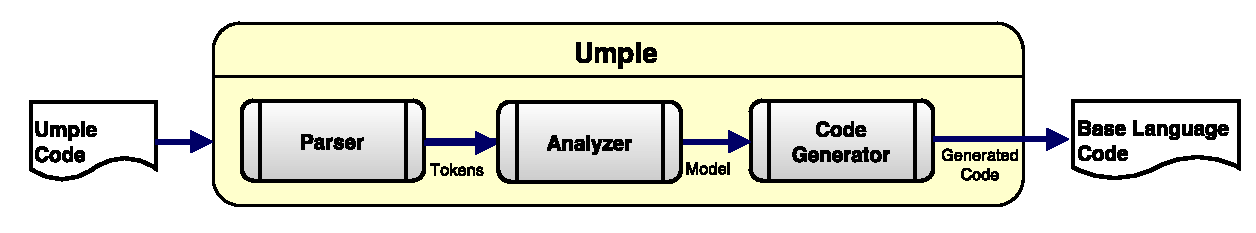
\includegraphics[width=0.99\textwidth]{Figures/umpleArchitecture.pdf} 
%\caption{Umple Architecture}
%\label{fig:umpleArchitecture}
%\end{figure}
%\centering
%\resizebox{\linewidth}{!}{Umple is available as an \textcolor{important} {Eclipse plugin}, \textcolor{important}{command-line} tool and \textcolor{important}{web-based} application. }
%\centering
%\end{frame}

\subsection{Transformations}
\begin{frame}
\frametitle{Transformations}
\begin{figure}[h]
\centering
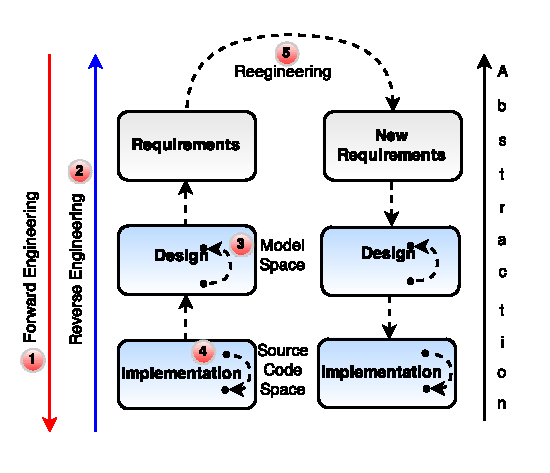
\includegraphics{Figures/transformationsRE}
\end{figure}
\end{frame}


\section{Motivations} 
\begin{frame}
\frametitle{Motivations}
Our desire to develop our reverse-engineering approach arose for two main reasons:

\begin{block}{Model-code duality}
End-product of umplification is not a separate model, but a single artifact seen as both the model and the code. 
\end{block}

\begin{block}{Improving Program Comprehension}
The resulting Umple code base tends to be simpler to understand as the abstraction level of the program has been `\textit{amplified}'.
\end{block}
\end{frame}

%------------------------------------------------
\section{Umplification}
%------------------------------------------------

\begin{frame}
\frametitle{Our Approach}
\centering
\textcolor{important}{\textbf{\large Umplification}}
\centering
A play on words with the concept of ‘\textit{amplification}’ and also the notion of converting into Umple. 
\newline
\begin{itemize}
	\item The approach produces a program with behavior identical to the original one, but written in Umple.
	\item The approach eliminates the distinction between code and model.
	\item The approach proceeds incrementally until the desired level of abstraction is achieved.
\end{itemize}
\end{frame}


\subsection{The Properties} 
\begin{frame}
\frametitle{The umplification approach is:}

\begin{block}{Incremental}
Proceeds incrementally until the desired level of abstraction is achieved
\end{block}

\begin{block}{Transformational}
Modeling constructs are added replacing the original code
\end{block}

\begin{block}{Interactive}
 Requires the user’s feedback in order to enhance the transformations.
\end{block}

\begin{block}{Extensible}
Uses a mechanism that can be readily extended to refine the transformations. 
\end{block}

\begin{block}{Implicit-Knowledge Conserving}
Preserves code comments, annotations, etc.
\end{block}
\end{frame}

%------------------------------------------------
%
%
%%------------------------------------------------
%\section{Reverse Engineering into Umple}
%%------------------------------------------------
%
%\begin{frame}
%\frametitle{Properties of the technique}
%
%\begin{block}{Incremental}
%\begin{itemize}
%\item It is performed in multiple small steps that profuce a small version of the system with a small amount of additional information
%\item At each step, the system remains compilable
%\item The approach proceeds incrementally until the desired level of abstraction is achieved
%\item These incremental transformations allow for user interaction to provide needed information that may be missing or hard to automatically obtain
%\end{itemize}
%\end{block}
%
%
%\begin{block}{Interactive}
%The user’s feedback may be used to en-hance the transformations.
%\end{block}
%
%\end{frame}
%\begin{frame}
%\frametitle{Properties of the technique (2)}
%
%\begin{block}{Extensible}
%It uses the set of transformation rules can be read-ily extended to refine the transformation mechanism. 
%\end{block}
%
%\begin{block}{Implicit-Knowledge Conserving}
%It preserves code comments, and, where possible, the layout of whatever code is not (yet) umplified. 
%\end{block}
%
%\begin{itemize}
%\item These properties allow developers to confidently umplify their systems without worrying about losing their mental model of the source code.
%\item Developers gain by having systems with a smaller body of source code that are intrinsically self-documented in UML. 
%\end{itemize}
%
%\end{frame}
%
%%------------------------------------------------


\subsection{The Umplification Process} 

\begin{frame}
\frametitle{The Umplification Process: Refactoring Steps}
The refactoring steps are the abstract transformations. The following are the refactorings steps currently implemented:

\begin{itemize}
\item\textbf{Transformation 0}: Initial transformation
\item\textbf{Transformation 1}: Transformation of generalization/specialization, dependency, and namespace declarations.
\item\textbf{Transformation 2}: Analysis and conversion of many instance variables, along with the methods that use the variables. 
	\begin{itemize}
	\item\textbf{Transformation 2a}: Transformation of variables to UML/\textbf{Umple attributes}.
	\item\textbf{Transformation 2b}: Transformation of variables in one or more classes to UML/\textbf{Umple associations}.
	\item\textbf{Transformation 2c}: Transformation of variables to UML/\textbf{Umple state machines}.
	\end{itemize}
\end{itemize}

\end{frame}

\begin{frame}
\frametitle{The Umplification Process: Refactoring Steps (2)}
As part of each transformation step, the accessor, mutator, iterator and event methods are adapted (refactored) to conform to the Umple generated methods.


\begin{itemize}
\item\textbf{Classes}:  None
\item\textbf{Inheritance}: None
\item\textbf{Attributes}: Accessor (getter) and mutator (setter) methods are removed/refactored from the original code. 
	
\item\textbf{Associations}: Accessor and mutator methods are removed or correctly injected into the umple code.

\item\textbf{State  Machines}: Methods triggering state change are removed if they are simple (just change state) or modified to call Umple-generated event methods. 
\end{itemize}
\end{frame}

%------------------------------------------------
\section{The Umplificator Technologies}
%------------------------------------------------

\subsection{General Requirements} 
\begin{frame}
\frametitle{General Requirements for the Umplificator Tool}
\begin{enumerate}
\item Support for various input languages

\item Incrementality

\item Rule execution control

\item Command-line support 

\item Directionality

\item Usability of Language
 
\item Rule organization

\item Output Export

\item Maintainability 

\item Extensibility
\end{enumerate}
\end{frame}

\subsection{Alternatives Approaches} 
\begin{frame}
\frametitle{Alternative Approaches studied - TXL}
\centering
\begin{figure}[h]
\centering
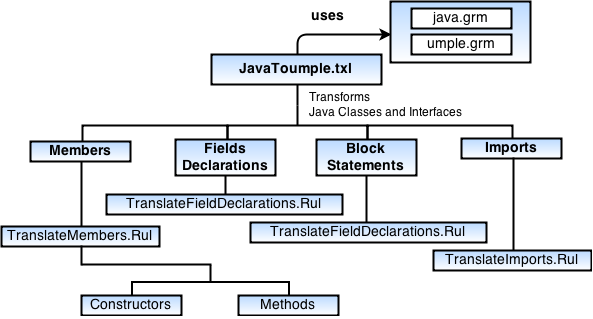
\includegraphics[width=0.98\textwidth]{Figures/TXLSTRUCTURE.png} 
\end{figure}
\end{frame}


\subsection{Alternatives Approaches} 
\begin{frame}
\frametitle{Alternative Approaches studied - ATL}
\centering
\begin{figure}[h]
\centering
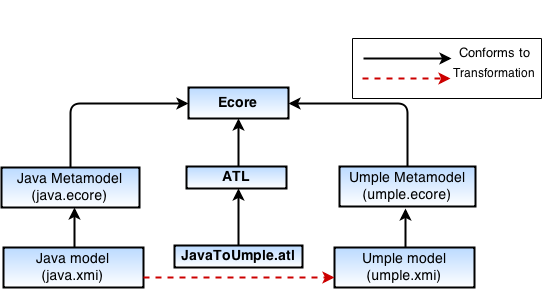
\includegraphics[width=0.75\textwidth]{Figures/ATLPROGRAM.png} 
\end{figure}
\end{frame}


\subsection{Comparison} 
\begin{frame}
\frametitle{ATL vs. TXL}

\begin{table}[h]
\centering
\begin{tabular}{l|p{2cm}|p{2cm}}
\toprule
\rowcolor[HTML]{BBDAFF}
\textbf{Evaluation Criteria} & \textbf{ATL}  & \textbf{TXL}   \\ \midrule
\textbf{Support for various input languages} & - &  +  \\ \hline
\textbf{Incrementality} & - &  +  \\ \hline
\textbf{Rule execution control} & + &   ++ \\ \hline
\textbf{Command-line support} & - & +++	    \\ \hline
\textbf{Usability of Language} & ++  & +   \\ \hline
\textbf{Rule organization} & +++ &  +++  \\ \hline
\textbf{Output Export} & - &  +++  \\ \hline
\textbf{Maintainability} & + &  ++  \\ \hline
\textbf{Extensibility} & - &  +  \\ 
\bottomrule
\end{tabular}
\end{table}
\end{frame}

%------------------------------------------------

\subsection{The Umplificator} 

\begin{frame}
\frametitle{Architecture}
\begin{figure}
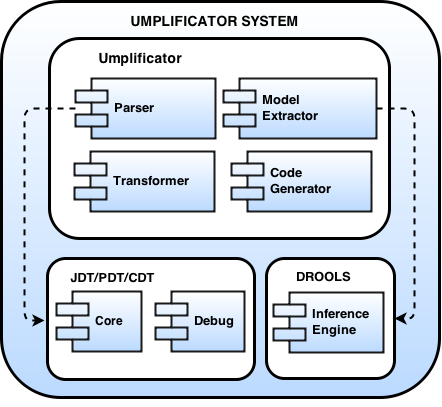
\includegraphics[width=0.6\linewidth]{Figures/UmplificatorComponents}
\end{figure}
\end{frame}


\begin{frame}
\frametitle{Third Party Technologies}

\begin{table}[h]
\begin{tabular}{l|l}
\toprule
\rowcolor[HTML]{BBDAFF}
\textbf{Technology} & \textbf{Targeted component(s)}   \\ \midrule
JDT/CDT/PDT  & Parser and Model Extractor \\ \hline 
Drools Rule Engine & Transformer  	 \\ \hline	
JOpt Simple & General  \\ \hline	
Log4j & General 	\\ \hline	
Perf4j & General  \\ \bottomrule
\end{tabular}
\end{table}
\end{frame}

\begin{frame}
\frametitle{The  Process Flow}
\centering
\begin{figure}
 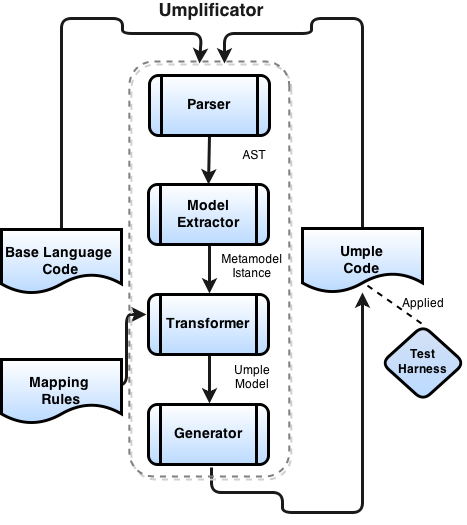
\includegraphics[width=0.5\linewidth]{Figures/Umplificator_ProcessFlow.png}
\end{figure}
\end{frame}
%------------------------------------------------

\subsection{Rule-Based Language} 
\begin{frame}[fragile] 
\frametitle{Rule-Based Language}

The rule engine interprets and executes the mapping rules on the source/target model to produce the umplified version of the target model.

\begin{lstlisting}[style=DroolsStyle]
rule "name"
  when LHS then RHS
end
\end{lstlisting}

A rule file in Drools is a file with a .drl extension that can have the following elements:

\begin{itemize}
\item \textbf{Package}
\item \textbf{Imports}
\item \textbf{Global Variables}
\item \textbf{Functions}
\item \textbf{Queries}
\end{itemize}
\end{frame}

\subsection{Summary} 
\begin{frame}[fragile] 
\frametitle{Summary of the Umplificator technologies}
The \textcolor{important}{\textbf{advantages}} of our mixed approach are: 

\begin{enumerate}
\item Separation of concerns
\item Speed and Scalability 
\item Centralization of Knowledge
\item Multi-level Testing 
\item Robust parsing
\item Efficiency 
\item Agile development 
\item Extensibility 
\item Reusability
\end{enumerate}

\end{frame}

\section{Evaluation}
%-----------------------------------------------
\subsection{Validation Phases} 
\begin{frame}[fragile] 
\frametitle{4-Phase Validation Process}

\begin{description}

\item[Testing Phase]: Unit testing.

\item[Pre-validation Phase] Validation with small Java systems written in high quality Java code. 

\item[Initial Phase]: Validation with Medium and large  open-source projects (\textbf{`training set'}).

\item[Machine Learning-Based Phase]: Validation with a set of randomly selected systems, the \textbf{`testing set'}.
\end{description}
\end{frame}


\subsubsection{Testing Phase} 
\begin{frame}[fragile] 
\frametitle{Testing Phase}
\textbf{135 tests that span all components of the tool} (parser, extractor, transformer, generator) and are run as part of our automated building process.
\begin{figure}[h]
\centering
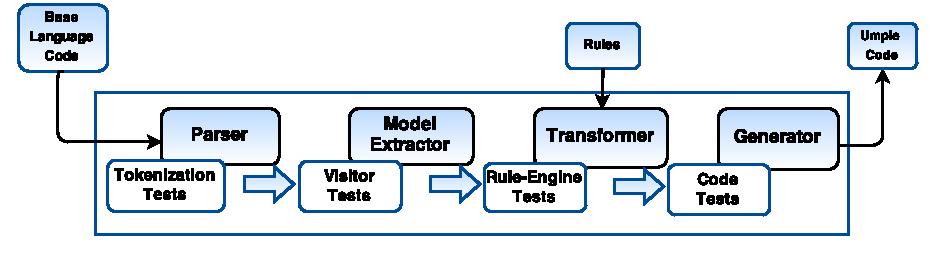
\includegraphics[width=1\textwidth]{Figures/testingPhase.pdf} 
\label{fig:testingPhase}
\end{figure}
\end{frame}

\subsubsection{Pre-Validation Phase} 
\begin{frame}[fragile] 
\frametitle{Pre-Validation Phase}
We have tested the umplificator using our own repository of \textbf{42 small Umple examples}.

\begin{figure}[h]
\centering
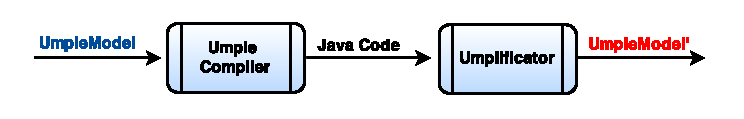
\includegraphics{Figures/preValidation.pdf} 
\label{fig:preValidation}
\end{figure}
\end{frame}

\subsubsection{Initial Validation Phase} 
\begin{frame}[fragile] 
\frametitle{Initial Validation Phase}
Apply the Umplificator to various \textcolor{important}{\textcolor{important}{open-source systems written in Java} that we have not created ourselves.} that we have not created ourselves.

\begin{table}
\label{table:umplifiedSystems}
\centering
\begin{tabular}{l|lrr}
\toprule
\rowcolor[HTML]{BBDAFF}
\textbf{Name} & \textbf{Version} & \textbf{LOC} & \textbf{\# of Classes} \\ \midrule
 1. JHotDraw                   & 7.5.1   & 82132   & 694      \\ 
\hline 2.  Weka      & 3.7.13  & 278642  & 1370        \\ 
\hline  3. Java Bug Reporting Tool 		& 1.0     & 2629    & 27        \\ 
\hline  4. JEdit                  	& 1.12    & 59699   & 84         \\ 
\hline  5. FreeMaker               & 2.3.15  & 39864   & 131         \\ 
\hline  6. Java Financial Library  		& 1.6.1   & 1248    & 28          \\ 
\hline  7. Args4j               	 & 2.0.30  & 2223    & 61            \\
\bottomrule
\end{tabular}
\end{table}
\end{frame}
%------------------------------------------------
\subsubsection{Results of Initial Validation}
%------------------------------------------------
\begin{frame}[fragile] 
\frametitle{Results of Initial Validation Phase - JHotDraw}

\begin{table}[h]
\centering 
\begin{tabular}{p{4cm}|rrrrr}
\toprule
\rowcolor[HTML]{BBDAFF}
\textbf{} & \textbf{TP}  & \textbf{FP} & \textbf{Expected} & \textbf{Precision}  & \textbf{Recall}\\ \hline
Attributes & 383  & 20  & 363  & 95\% & 100\% \\ \hline
Associations optional-one-to-many &  22 & 0 & 49 & 100\% & 45\% \\ \hline
Associations optional-one-to-one &  115 & 0 & 185  & 100\% & 62.2\% \\ \hline
Associations many-to-many & 30 & 0 & 32 & 100\% & 93.8\%\\ \bottomrule
\end{tabular}
\end{table}
\end{frame}
%
%\begin{frame}[fragile] 
%\frametitle{Results of Initial Validation Phase - Weka}
%\begin{table}[h]
%\centering 
%\begin{tabular}{p{4cm}|rrrrr}
%\toprule
%\rowcolor[HTML]{BBDAFF}
%\textbf{} & \textbf{TP}  & \textbf{FP}  & \textbf{Expected} & \textbf{Precision}  & \textbf{Recall}\\ \hline
%Attributes & 1281	& 0	& 1510 & 100\%	& 84.9\% \\ \hline
%Associations optional-one-to-many &  168 & 0 & 442 & 100\% & 38\% \\ \hline
%Associations optional-one-to-one &  224 & 12 & 285 & 94.92\%  & 86.8\% \\ \hline
%Associations many-to-many & 89 & 0 & 115 & 100\% & 77.4\% \\ \bottomrule
%\end{tabular}
%\end{table}
%\end{frame}
%
%\begin{frame}[fragile] 
%\frametitle{Results of Initial Validation Phase - Args4j}
%\begin{table}[h]
%\centering 
%\begin{tabular}{p{4cm}|rrrrr}
%\toprule
%\rowcolor[HTML]{BBDAFF}
%\textbf{} & \textbf{TP}  & \textbf{FP} & \textbf{Expected}  & \textbf{Precision}  & \textbf{Recall}\\ \hline
%Attributes & 186 & 5 & 186 & 97.4\% & 100\%  \\ \hline
%Associations optional-one-to-many &  12 & 0 & 12 & 100\% & 100\%\\ \hline
%Associations optional-one-to-one &  4 & 0 & 5  & 100\% & 100\% \\ \hline
%Associations many-to-many & 28 & 0 & 28 & 100\% & 100\% \\ \bottomrule
%\end{tabular}
%\end{table}
%\end{frame}

\begin{frame}[fragile] 
\frametitle{Results of Initial Validation Phase - Execution Time}
\begin{table}[h]
\centering
\begin{tabular}{p{4cm}|rr}
\toprule
\rowcolor[HTML]{BBDAFF} 
  & \multicolumn{2}{l}{\textit{\textbf{Execution Time (in ms)}}} \\\hline
\textbf{Component}             & \textbf{JHotDraw}     & \textbf{Args4J}   \\\hline
\textbf{Parsing}               & 50899  & 12500         \\\hline
\textbf{Extractor}             & 21025  & 3204         \\\hline
\rowcolor{yellow} 
\textbf{Transformer}           & 339327 & 920          \\\hline
\textbf{Generating Umple Code} & 1700   & 450          \\\hline
\textbf{Total Time:}           & 412951 & 14074        \\\hline
\end{tabular}
\end{table}
\end{frame}

%------------------------------------------------
%------------------------------------------------
\subsubsection{Second Validation Phase}
%------------------------------------------------
\begin{frame}[fragile] 
\frametitle{Second Validation Phase}
\begin{enumerate}
\item \textcolor{important}{\textbf{Download}} 100 projects (randomly).
\item \textcolor{important}{\textbf{Umplify}} the projects.
\item \textcolor{important}{\textbf{Report}} the scores.
\begin{itemize}
\item (Doesn't Exist) 
\item F.Umplify.Score.log 
\item \{012\}.Umplify.Score.log 
\end{itemize}
\end{enumerate}
\end{frame}

\section{Case Studies}
\subsection{JHotDraw} 

\begin{frame}
\frametitle{JHotDraw}

\begin{figure}[h]
\centering
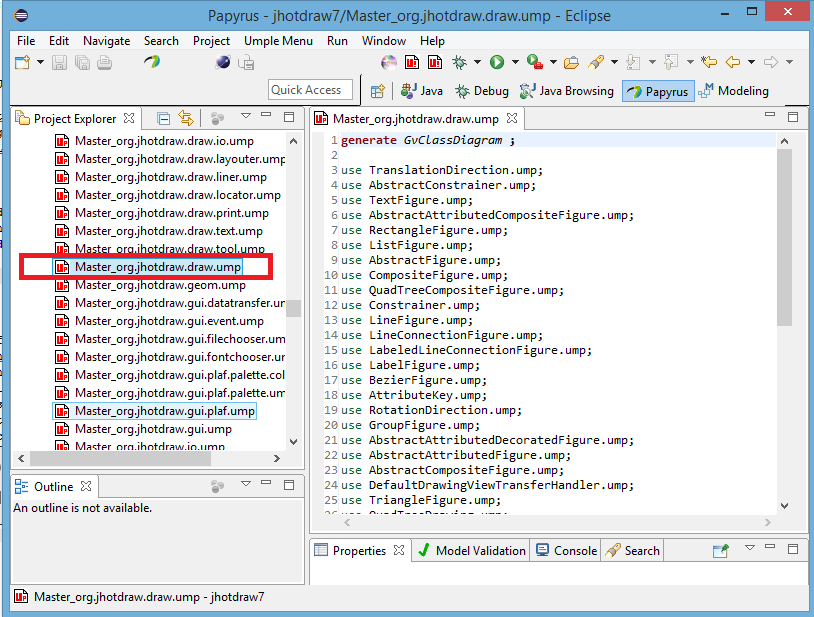
\includegraphics[width=0.80\textwidth]{Figures/jhotdrawMasterDraw.png} 
\end{figure}
\end{frame}

\begin{frame}
\frametitle{JHotDraw}
\begin{figure}[h]
\centering
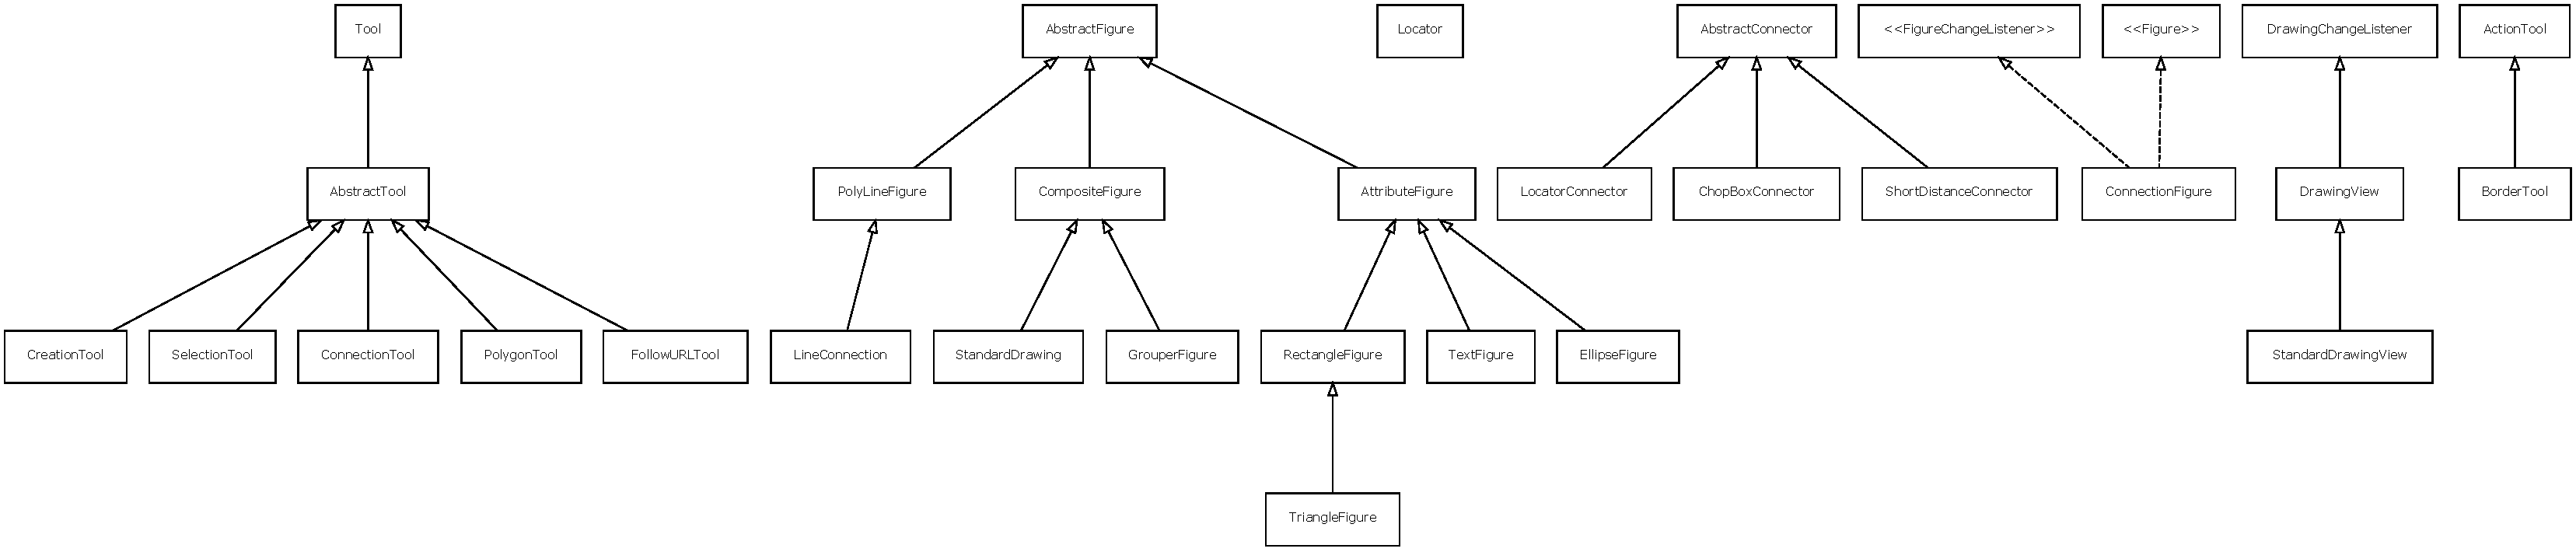
\includegraphics[width=0.99\textwidth]{Figures/jhotdrawuml.pdf} 
\end{figure}

\end{frame}

%------------------------------------------------

\subsection{WEKA} 

\begin{frame}
\frametitle{WEKA}
\begin{block}{Results}
Initial Umplification results for Weka nonetheless had a precision of 85\% when it comes to attributes and 38\% for 1-to-many associations.
\end{block}

\begin{block}{Why}
Note that a precision of 38\% doesn't mean that the Umplificator has missed 62\% associations of this type. It means that some of them were not correctly transformed into Umple (e.g. incorrect navigability, role names or transformation of accessor/mutator methods).
\end{block}
\end{frame}


\begin{frame}
\frametitle{Args4j  - Modernization}

\begin{itemize}
\item \textbf{Original} Args4j Java source code is composed of 61 classes and 2223 lines of code.
\item \textbf{Umplified} Args4j source code is composed of 122 (2 per input class) umple files and 1980 lines of code in total.
\item Total number of lines of code in files containing modeling constructs (X.ump) is 312 LOC.
\item Total number lines of code in files with algorithmic/logic code (X\_code.ump) is 1668 LOC. If we exclude the umple class declarations and curly brackets, the number becomes 1424 LOC.
\end{itemize}

\begin{block}{Translating source code base}
To achieve the goal of translating Args4j into C++, a developer must translate 1518 lines of code (rather than 2223 lines of code). 
\end{block}
\end{frame}
%------------------------------------------------

%------------------------------------------------

\subsection{Tuning of the Umplificator} 
\begin{frame}
\frametitle{Tuning of the Umplificator}
The complexity of the tuning depends on the number of false positives and false negatives that the tool generates.

%\begin{enumerate}
%  \item If there is an Umple construct that was missed from the extraction (false negative), we may add a new mapping rule to cover this case.
%  \item If there is an Umple construct that was incorrectly identified (false positive), we may edit the corresponding mapping rule.
%  \item If one of the methods requiring additional transformations (as described in Table 1) was incorrectly refactored, we may review and correct the refactoring action (a function in Drools language) that led to the incorrect piece of code.
%\end{enumerate}
\begin{enumerate}
  \item \textbf{Umple construct  missed  (false negative)}: we may add a new mapping rule to cover this case.
  \item \textbf{Umple construct  incorrectly identified (false positive)}: we may edit the corresponding mapping rule.
  \item \textbf{Method  incorrectly refactored}: we may review and correct the refactoring action (a function in Drools language) that led to the incorrect piece of code.
\end{enumerate}
\end{frame}

%------------------------------------------------
\section{Related Work}
%------------------------------------------------
\begin{frame}
\begin{table}[ht]
\frametitle{Related Work}
\centering
\begin{tabularx}{\textwidth}{X|lllllll}
\toprule
\rowcolor[HTML]{BBDAFF}
\textbf{Author-Ref}  & \rotatebox{90}{\textbf{Scalability}} & \rotatebox{90}{\textbf{Incrementality}}& \rotatebox{90}{\textbf{Validation}}& \rotatebox{90}{\textbf{Usability}}& \rotatebox{90}{\textbf{Target Lang.}} & \rotatebox{90}{\textbf{Attributes?}}& \rotatebox{90}{\textbf{Associations?}} \\ \hline
Barowski et al. - 2002  & N & N & P & N & Java  & P & P \\ \hline
Grant et al. - 2011  & P  & N & P &  F & Java  & F & P \\ \hline
Gueeheneuc - 2004  & P & P& F  & F &Java  & F & F \\ \hline
Vinita et al. - 2008  & N & N & N & N & Cpp & P & P \\ \hline
Kang et al. - 2007  & N & N& N & F &Java & F & P \\ \hline
Sutton et al. - 2007  & N & N & P & F & Cpp & F & F\\ \hline
Korshunova et al. - 2006  & P & N & P & F & Cpp & F & P\\ \hline
{Umplification} & \textbf{P} & \textbf{F} & \textbf{P}  & \textbf{F} & \textbf{Java,Cpp} & \textbf{F} & \textbf{P} \\ 
\hline
\end{tabularx}
\end{table}
\end{frame}

%------------------------------------------------
\section{Conclusions and Future Work}
%------------------------------------------------

\begin{frame}
\frametitle{Summary of Contributions}
\begin{enumerate}
\item The overall concept of umplification and the defined levels of refactoring;

\item An understanding of how umplification compares with other reverse engineering techniques;

\item The implementation and analysis of integrating different transformation technologies;  resulting in the Umplificator tool itself;

\item Case studies of Umplification, demonstrating strengths, weaknesses and opportunities. Results presented in this thesis are reproducible and repeatable; 

\item Mapping rules for Umplification and the language for expressing these;

\item Detection of associations in a body of source code;

\item **{\scriptsize We also made improvements to Umple compiler  to support abstract classes, interfaces and top-level enumerations, as needed to support the case studies.}**
\end{enumerate}
\end{frame}

\section{Tools Developed}
\begin{frame}
\frametitle{Summary of Tools Developed}
\textcolor{important}{\textbf{Command Line Tool}}
\begin{enumerate}
\item \textbf{cruise.umplificaror.eclipse\_vX.X.X.jar} : Plug-in for the Eclipse IDE 
\item \textbf{umplificator\_X.Y.Z.jar} : Command-Line tool for umplification 
\item \textbf{validator\_X.Y.Z.jar} : Command-Line tool that checks whether the input Umple code generates compilable base language code. 
\end{enumerate}

Umplifying source code by means of the command-line tool can be done using the following command:
\newline

\textbf{java -jar umplificator.jar inputFile \textcolor{important}{-level}=\textcolor{red}{1,2,3} \textcolor{important}{-splitModel -dir -path}}
\end{frame}

\begin{frame}
\frametitle{Summary of Tools Developed}
\textcolor{important}{\textbf{Web-App}}
\begin{figure}[h]
\centering
\frame{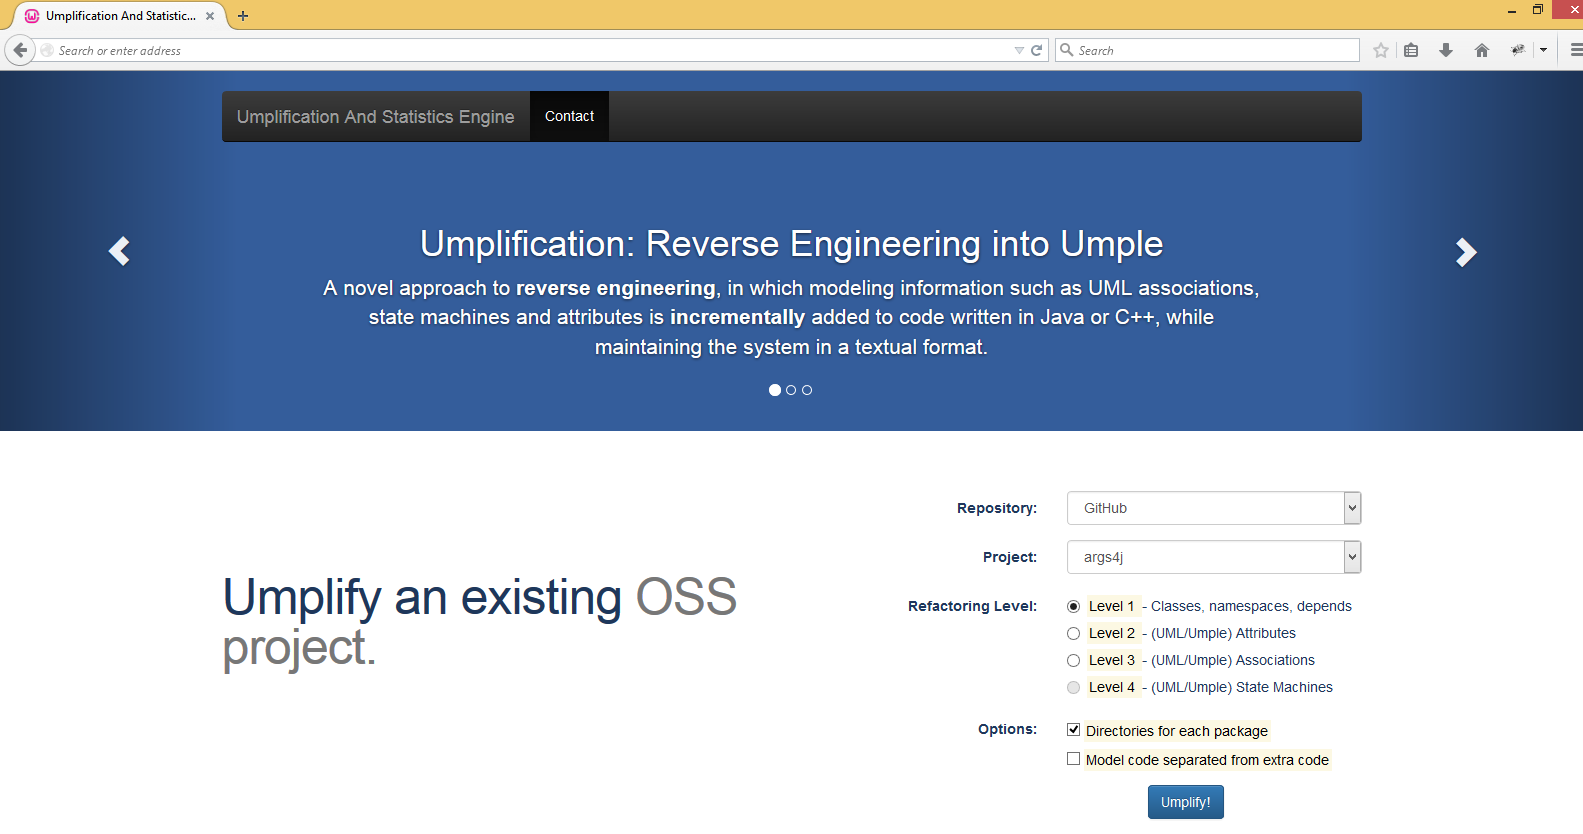
\includegraphics[width=0.98\textwidth]{Figures/UmplificatorOnline.png}}
\end{figure}
\end{frame}

\begin{frame}
\frametitle{Summary of Tools Developed}
\textcolor{important}{\textbf{Various}}
\begin{block} {Script}
The code for the script is published online and can be found in our \textbf{code repository} in the following directory:

\url{cruise.umplificator/scripts/umplificator_all_projects.sh}.
\end{block}
\begin{block} {Downloader}
The project surrounding the umplificator that automatically downloads, tracks and reports on various projects can be found at: 

\url{https://github.com/mgarzon/dlproj}.
\end{block}
\end{frame}

\begin{frame}
\frametitle{Future Work}
\begin{enumerate}
\item {\large Umplify more Projects}
\item {\large State Machines Support} 
\item {\large IDE Integration}
\item {\large Evaluation with real developers}
\item {\large Exploring other types of software}
\item {\large Umplifying code that matches other model elements}
\end{enumerate}
\end{frame}

\begin{frame}
\frametitle{The End}
\centering
\LARGE{\textcolor{important}{Thank you!}}
\end{frame}


%------------------------------------------------
\section{Additional Notes}
%------------------------------------------------
\begin{frame}
\centering
\textcolor{important}{{\fontsize{40}{50}\selectfont Additional Notes}}
\end{frame}

\begin{frame}
\frametitle{Answers to Research Questions (1)}
\textcolor{important}{\textbf{RQ1. To what extent can we achieve automated umplification?}}
\begin{enumerate}
\item The evaluation results showed that our approach and its current implementation are effective and efficient enough to be applied to real systems. 
\item We were able to successfully umplify many real open-source systems at varying degrees of effectiveness, and were able to iteratively improve this effectiveness by adjusting rules.
\end{enumerate}
\end{frame}

\begin{frame}
\frametitle{Answers to Research Questions (2)}
\textcolor{important}{\textbf{RQ2. What transformation technology and transformations  will work effectively for umplification?}}
\begin{enumerate}
\item We discussed our experiments with ATL and TXL approaches.
\item We selected an approach that uses: 
	\begin{enumerate}[(a)] 
	\item \textbf{the mature xDT} family of parsing libraries (JDT, CDT, etc.) to process both code and 			   textual models, and build in memory models;
	\item the \textbf{Drools tool} to transform the in-memory models, accomplishing the core umplification   task and;
	\item \textbf{our own generator technology} to produce revised versions of the system.
	\end{enumerate}
\end{enumerate}
\end{frame}

\begin{frame}
\frametitle{Answers to Research Questions (3)}

\textcolor{important}{\textbf{RQ3. What should be the architecture, design and implementation of an umplification tool?}}
The advantages of the selected approach enabled the following aspects, each of which we discussed in Chapter 5:

\begin{enumerate}

\item Separation of concerns
\item Speed and Scalability
\item Centralization of Knowledge
\item Multi-level Testing
\item Robust parsing 
\item Efficiency
\item Agile development 
\item Extensibility
\item Reusability
\end{enumerate}

\end{frame}

\begin{frame}
\frametitle{Answers to Research Questions (4) }
\textcolor{important}{\textbf{RQ4. What would be an effective process for improving the accuracy of the umplification tool?}}
\begin{enumerate}
\item An approach adapted from the model often used in machine learning considerably improved the precision and recall of our transformations.
\item This validation approach takes one set of systems as the \textcolor{important}{`\textbf{training set}'} and then takes another set as the \textcolor{important}{\textbf{`testing set'}} to see how well the Umplificator performs on unknown systems. 
\item The Umplificator is tuned based on problems found when working with the testing set. 
\end{enumerate}
\end{frame}

%------------------------------------------------
\begin{frame}
\frametitle{The Umple Architecture}
\begin{figure}[h]
\centering
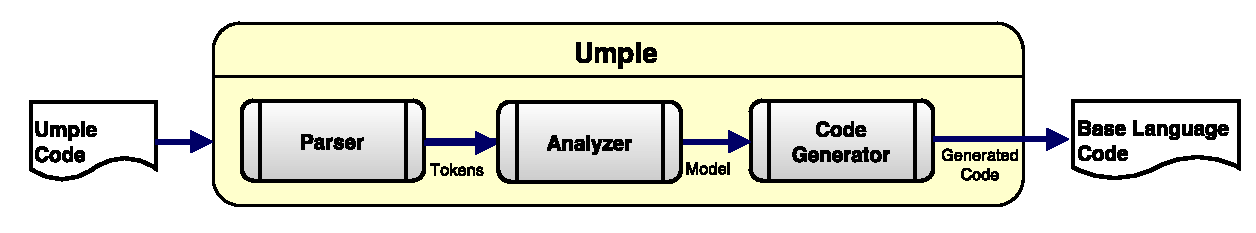
\includegraphics[width=0.99\textwidth]{Figures/umpleArchitecture.pdf} 
\caption{Umple Architecture}
\label{fig:umpleArchitecture}
\end{figure}
\centering
\resizebox{\linewidth}{!}{Umple is available as an \textcolor{important} {Eclipse plugin}, \textcolor{important}{command-line} tool and \textcolor{important}{web-based} application. }
\centering
\end{frame}

\begin{frame}[fragile] 
\frametitle{EXAMPLE}
\begin{enumerate}
    \item \textbf{Task:}  \emph{Umplify} a small system written in Java.
    \item \textbf{Initial Input:} Three Java Classes  \emph{(Student.java, Person.java, Mentor.java}).
    \item \textbf{Final Output:} An \emph{Umple model} containing three Umple Classes (which contain Umple Attributes, associations, etc).
	\begin{itemize}
	   \item This Umple Model can also be viewed and edited as an UML Class Diagram.
	\end{itemize}
\end{enumerate}

\end{frame}

%------------------------------------------------
\begin{frame}[fragile] 
\frametitle{Tranformations 0 and 1 (Student.java)}
\begin{itemize}
  \item One-to-one direct and simple mappings between constructs.
  \item The final output after execution, is an Umple model/program that can be compiled.
  \item Three files created at this point:  \emph{Student.ump, Mentor.ump, Person.ump}. 
\end{itemize}
\underline{Java code:}
\begin{lstlisting}[style=JavaStyle]
package university;
import java.util.*;
public class Student extends Person { ... more code }
\end{lstlisting}
\underline{Umple code:}
\begin{lstlisting}[style=UmpleInStyle]
namespace university;
class Student { 
   depend java.util.*;
   isA Person;
  /*The rest of the code*/
}
\end{lstlisting}

\end{frame}

\begin{frame}
\frametitle{UML Class Diagram After Tranformation 1}
\begin{figure}
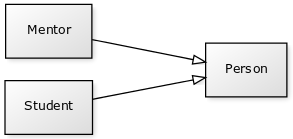
\includegraphics[width=0.8\linewidth]{Figures/uml1.png}
\end{figure}
\end{frame}

%------------------------------------------------

%------------------------------------------------
\begin{frame}[fragile] % Need to use the fragile option when verbatim is used in the slide
\frametitle{Transformation 2: Refactoring to Create Attributes}
\begin{itemize}
  \item We analyze all instance variables for their presence in constructor and get/set methods.
\begin{table}[h]
\begin{tabular}{@{}cccc@{}}
\toprule
\rowcolor[HTML]{BBDAFF} 
Constructor & Setter & Getter & \begin{tabular}[c]{@{}c@{}}Attribute\\ (probability)\end{tabular} \\ \midrule
Yes         & Yes    & Yes    & High                                                              \\
Yes         & Yes    & No     & Low                                                               \\
Yes         & No     & Yes    & High                                                              \\
Yes         & No     & No     & Low                                                               \\
No          & Yes    & Yes    & High                                                              \\
No          & Yes    & No     & Low                                                               \\
No          & No     & Yes    & Medium                                                            \\
No          & No     & No     & Medium Low                                                        \\ \bottomrule
\end{tabular}
\end{table}
  \item We culminate this refactoring step by removing or refactoring getters and setters of the previously identified attributes.
\end{itemize}
\end{frame}

%------------------------------------------------

%------------------------------------------------
\begin{frame}[fragile] % Need to use the fragile option when verbatim is used in the slide
\frametitle{Refactoring to Create Attributes - The Input code}
\underline{Umple code after transformation 1 (INPUT): }

\begin{lstlisting} [style=UmpleInStyle]
class Student { 
 depend java.util.*;
 isA Person;
 public Mentor mentor; 
 public static final int  MAX_PER_GROUP = 10;
 private int id;
 private String name; 
 private boolean isActive;
 
 public Student(int id,String name){
     id = id; name = name;
 }
 public String getName(){ 
  String aName = name;
  if (name == null) { throw new  RuntimeException("Error");} 
  return aName;
}  
\end{lstlisting}
\end{frame}

\begin{frame}[fragile] % Need to use the fragile option when verbatim is used in the slide
\frametitle{Refactoring to Create Attributes - The Input code}

\begin{lstlisting} [style=UmpleInStyle]
public Integer getId() { 
   return id; 
} 
public void setId (Integer id) {    
   this.id = id;
}	
public boolean getIsActive() { 
   return isActive;
}
public void setIsActive ( boolean  aIsActive) {
  isActive = aIsActive;
}
public Mentor getMentor() { return mentor; } 
public void setMentor(Mentor mentor) { this.mentor = mentor; } 
}
} 
\end{lstlisting}
\end{frame}

\begin{frame}[fragile] % Need to use the fragile option when verbatim is used in the slide
\frametitle{Refactoring to Create Attributes - Analyzing the code:}
%  We  analyze the member variables to determine:
%\begin{enumerate}
%  \item  Is the field present in the parameters of the constructor?
%  \item  Does the field possess a getter?
%  \item  Does the field possess a setter?
%  \item Is the field’s type, a primitive type?
%\end{enumerate}
For the class Student, we obtain the following results:
\begin{table}[h]
\begin{tabular}{@{}lcccc@{}}
\toprule
\rowcolor[HTML]{BBDAFF} 
\textbf{\begin{tabular}[c]{@{}l@{}}Member\\ Variable\end{tabular}} & \textbf{Constructor?} & \textbf{Getter?} & \textbf{Setter?} & \textbf{Type?} \\ \midrule
\textbf{id}                                                        & Yes                   & Yes              & Yes              & Yes            \\
\textbf{isActive}                                                  & No                    & Yes              & Yes              & Yes            \\
\textbf{name}                                                      & Yes                   & Yes              & No               & Yes            \\
\textbf{MAX\_PER\_GROUP}                                           & No                    & No               & No               & Yes           
\end{tabular}
\end{table}
\end{frame}


\begin{frame}[fragile] % Need to use the fragile option when verbatim is used in the slide
\frametitle{Refactoring to Create Attributes- The Output code}
\underline{Umple code after transformation 2a (OUTPUT): }
\begin{lstlisting} [style=UmpleOutStyle]
class Student { 
 Integer id;
 lazy Boolean isActive;  
 immutable name;
 const Integer MAX_PER_GROUP = 10;
 after getName { 
  if (name == null) { 
   throw new 
     RuntimeException("Error");}
 }
 /*DEVELOPER CODE - PROVIDED AS-IS*/
  public Mentor mentor; 
  public Mentor getMentor() { return mentor; } 
  public void setMentor(Mentor mentor)
  { 
     this.mentor = mentor; 
  } 
}

\end{lstlisting}
\end{frame}

\begin{frame}
\frametitle{UML Class Diagram After Tranformation 2a.}
\begin{figure}
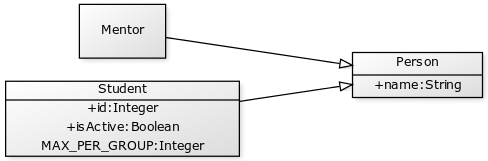
\includegraphics[width=0.99\linewidth]{Figures/uml2.png}
\end{figure}
\end{frame}

%------------------------------------------------

%------------------------------------------------
\begin{frame}[fragile] % Need to use the fragile option when verbatim is used in the slide
\frametitle{Refactoring to Create Associations}
\begin{itemize}
  \item In order to guarantee the correct extraction of an association and to avoid false-negative cases, we consider not only the getter and setter of the fields but also the iteration call sequences (iterators). 
  \item A variable represents an association if all of the following conditions apply:
\begin{enumerate}
  \item Its declared type is a \textbf{ Reference type} (generally a class in the current system).
  \item The variable field is simple, or the variable field is a container (also known as a collection).
  \item The class in which the variable is declared, stores, access and/or manipulates instances of the variable type.
\end{enumerate}
\end{itemize}

\end{frame}

\begin{frame}[fragile] % Need to use the fragile option when verbatim is used in the slide
\frametitle{Refactoring to Create Associations (2)}
\underline{Umple code before transformation 2b (INPUT): }

\begin{lstlisting}[style=UmpleInStyle]
class Student {/*The rest of the code*/ } 

class Mentor { 
 depend java.util.Set; 
 isA Person;
 public Set<Student> students; 
 public Set<Student> getStudents()  
  { return students; } 

 public void  setStudents (Set<Student>students) 
  { this.students = students; } 

 public void addStudent( Student  aStudent) 
  { students.add(aStudent); }

 public void removeStudent(Student   aStudent)
  { students.remove(aStudent);}
} 

\end{lstlisting}

\end{frame}

\begin{frame}[fragile] % Need to use the fragile option when verbatim is used in the slide
\frametitle{Refactoring to Create Associations (3)}
\underline{Umple code after transformation 2b (OUTPUT): }
\begin{lstlisting}[style=UmpleOutStyle]

class Mentor {
 0..1 -- 0..* Student; 
}
class Student {/*The rest of the code*/}

\end{lstlisting}
\end{frame}


\begin{frame}
\frametitle{UML Diagram After Tranformation 2b.}
\begin{figure}
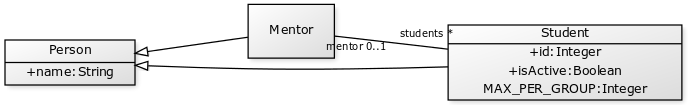
\includegraphics[width=0.99\linewidth]{Figures/uml3.png}
\end{figure}
\end{frame}

\end{document} 